% The final version needs to be converted to word (or other related format)
% so there's no point in spending a huge amount of time getting everything
% looking perfect in this document.  But it will be much easier for us to
% collaborate with latex rather than word.
%
% Pages 10-15
% Due: 31 Dec 08 !!
% 
% Want lots of graphics and illustrative code samples
% All graphics need to work in black & white


\documentclass[oneside]{article}
\usepackage{fullpage}
\usepackage[pdftex]{graphicx}
\graphicspath{{graphics/}}
\DeclareGraphicsExtensions{.png,.pdf}
\usepackage{hyperref}
\usepackage{verbatim}
\renewcommand\rmdefault{bch}
\usepackage[small]{caption}
\usepackage[tiny]{titlesec}
\titlelabel{}
\linespread{1.07} 

\usepackage[round,sort&compress,sectionbib]{natbib}
\bibliographystyle{plainnat}

\title{Beautiful data: The housing crisis in CA}
\author{Deborah F. Swayne and Hadley Wickham}
\date{\today}

\raggedbottom

\begin{document}
\maketitle 

\section{Introduction}

Motivation: housing crisis.  Can we use housing sale data to quantify it more accurately?  How do our findings compare to findings reported by the media?  Can we locate market segments that were particularly badly hit?

All data and code is available from our git repository - \url{https://github.com/hadley/sfhousing}.  You can see some of the false starts that we made.  Both code and data are licensed with the MIT license. We'll illustrate snippets of code here: you probably won't be familiar with R, but you should still be able to get the gist of it.  Mention the file name next to each section in which it is used.

\section{How did we get the data?}

Like many of our for fun data explorations, this all started when we discovered an interesting data source: the weekly housing sales data provided by the SF Chronicle (\url{}). We had initially planned on scraping the data off the website, but a little detective work revealed that the data is already available in a machine readable form. 

For each week, there was a text file containing all of the data in the following form:

\begin{verbatim}
rowid: 1
county: Alameda County
city: Alameda
newcity: 1
zip: 94501
street: 1220 Broadway
price: $509,000
br: 4
lsqft: 4420
bsqft: 1834
year: 1910
\end{verbatim}

Each file was available at a url of the form \url{http://www.sfgate.com/c/a/year/month/day/REHS.tbl}.  We used R to generate a sequence of Sunday's from the first on record, 2003-04-27, which we found with a little more detective work, to the most recent.  With those dates in hand, we made a list of all the urls and then used the command line tool {\tt wget} to download them all.   We used wget because of it's support for resuming where it left off.  If our internet connection went down or we moved our laptop to another network we didn't need to worry about starting for scratch.  Saves a lot of time!

The next step was to get the data into a more standard format: we chose csv because each file had (approximately) the same fields, and it's a format that all statistical packages (and excel etc) can import and export.  This isn't a standard data format, but nevertheless it's fairly easy to write a parser to deal with it.  This gives us a file like follows:

\begin{verbatim}
county,city,zip,street,price,br,lsqft,bsqft,year,date,datesold
Alameda County,Alameda,94501,1220 Broadway,509000,4,4420,1834,1910,2003-04-27,NA
Alameda County,Alameda,94501,429 Fair Haven Road,504000,4,6300,1411,1964,2003-04
-27,NA
Alameda County,Alameda,94501,2804 Fernside Boulevard,526000,2,4000,1272,1941,200
3-04-27,NA
Alameda County,Alameda,94501,1316 Grove Street,637000,3,2700,1168,1910,2003-04-2
7,NA
\end{verbatim}

This is a less human readable, but it's a very standard format that practically any tool can read in.  Another minor advantage of this more compact form (not repeating the field names all the time) was reduced storage requirements: 88 vs 45 meg.  Note that R uses {\tt NA} to represent missing values.

Takes just a few minutes to parse all 293 data files.  But a few hours tweaking the parser to get all the edge cases.  Things like stripping \$ and , out of prices to get a number.  And parsing the sold dates, which weren't in a totally consistent format.

Total of 521,726 records.  Had to update mid-way throughout analysis procedure to get the latest data.  This is where having a well though-out script really helps.  Very common in real-life statistical analysis: data is always changing because new data is collected, or old data is corrected.  

\section{Geocoding} 

How to geocode 400,000 addresses?  

Web services - google, yahoo - restrictive licensing clauses.

UCGS.  How long it look to geocode them all.  Send paragraph to Dan Goldberg to check for accuracy.  Never hurts to spend a lot of time checking the data at this level as everything else depends on it.  However, will omit a lot of the work we did because it's more interesting to talk about the findings.

Bar chart showing address quality.  Make sure to have percent on the y-axis.  Won't throw out bad matches right away, because we need varying levels of accuracy for different purposes: city level accuracy is fine when we are comparing cities, will want address level when we are looking within a city, or focusing on purely geographical comparisons.

\section{Analysis}

We'll start by looking at number of sales and average prices over all of California, and then zoom into focus on regions of interest.  Finally, we'll look at a few plots that reveal features of the data that allow us to investigate other housing patterns in California.

\begin{figure}[htbp]
  \centering
    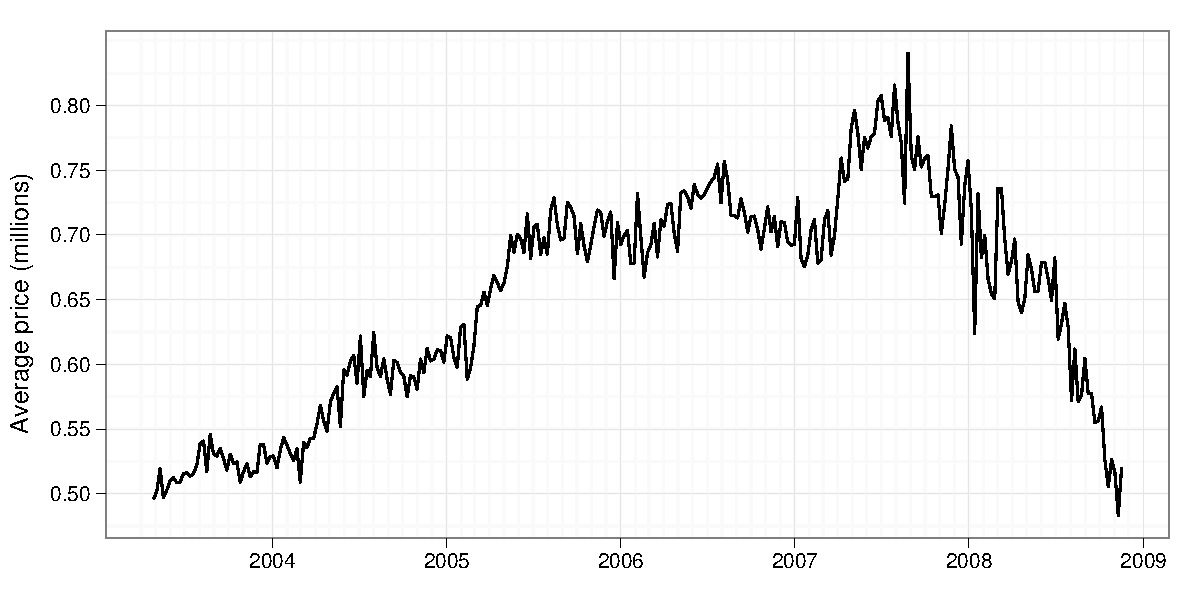
\includegraphics[width=0.5 \linewidth]{daily-price}%
    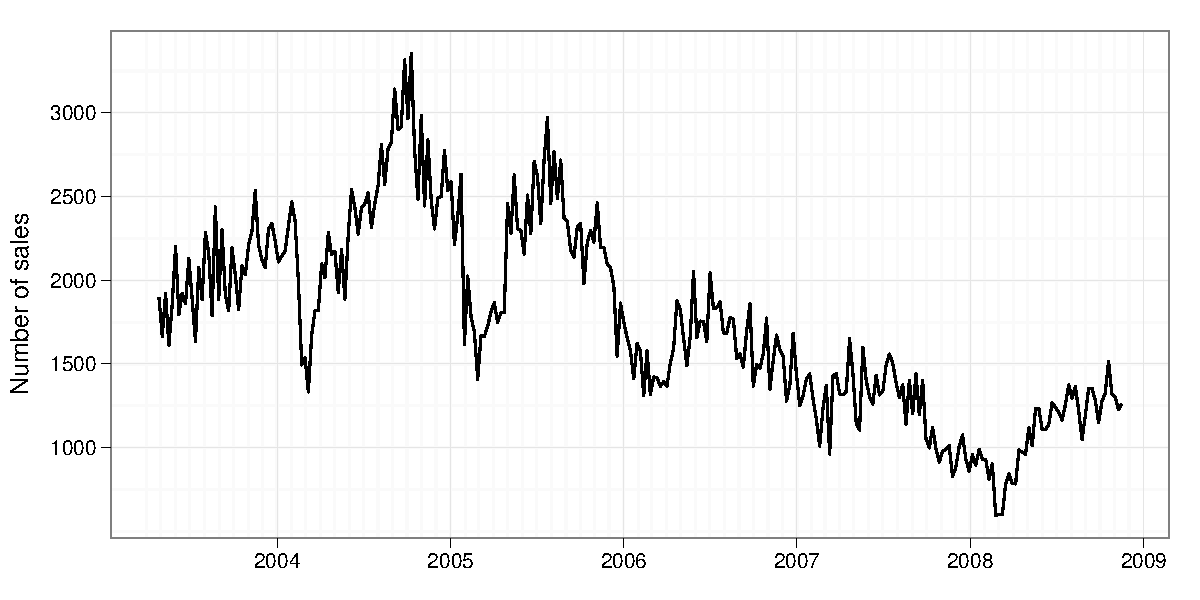
\includegraphics[width=0.5 \linewidth]{daily-sales}
  \caption{Daily average prices (right) and sales (left)}
  \label{fig:daily}
\end{figure}

Figure~\ref{fig:daily} shows average daily sales and prices over the course of the data.  The effect of the housing crisis is striking in the average sale prices, with an increasing trend until June 2007 and then a rapid decrease.  Sales show a different pattern.  We see a gradual decrease in number of sales from mid 2006, and then an increasing trend in early 2008. Maybe this is because of people buying foreclosed houses?  We'll look at that in more detail later on.

\subsection{Adjusting for inflation}

CPI data - \url{http://www.bls.gov/CPI}.  This is a common theme in data analysis: we need to combine our original data with new data that provides context and helps us understand it better.  In this case, we want to control for changes in relative buying power (i.e.\ inflation).  Even over this relatively short time span it's a bad idea to ignore inflation: \$1\,000 2004 dollars, would be worth\$1\,170 today.

We used the CPI time series for the West coast.

Figure~\ref{fig:inflation} shows the CPI-based inflation measurement and the affected of adjusting for inflation.  Failing to adjust for inflation makes the increasing trend prior to mid 2007 look more pronounced.  All prices in the remainder of this paper will be inflation adjusted.

\begin{figure}[htbp]
  \centering
    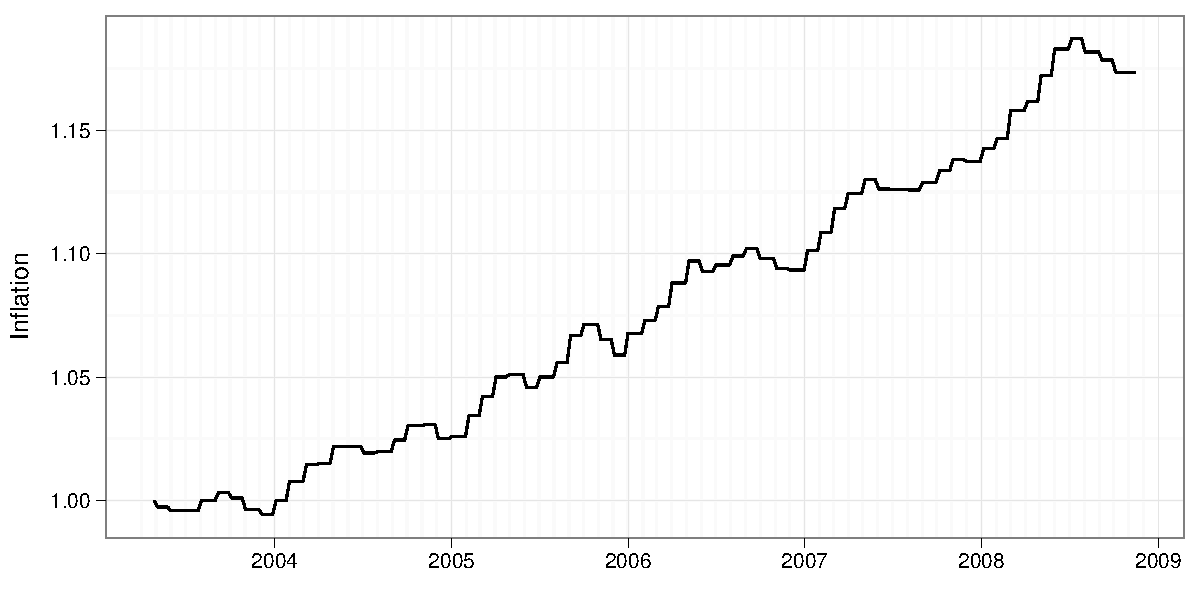
\includegraphics[width=0.5 \linewidth]{daily-cpi}%
    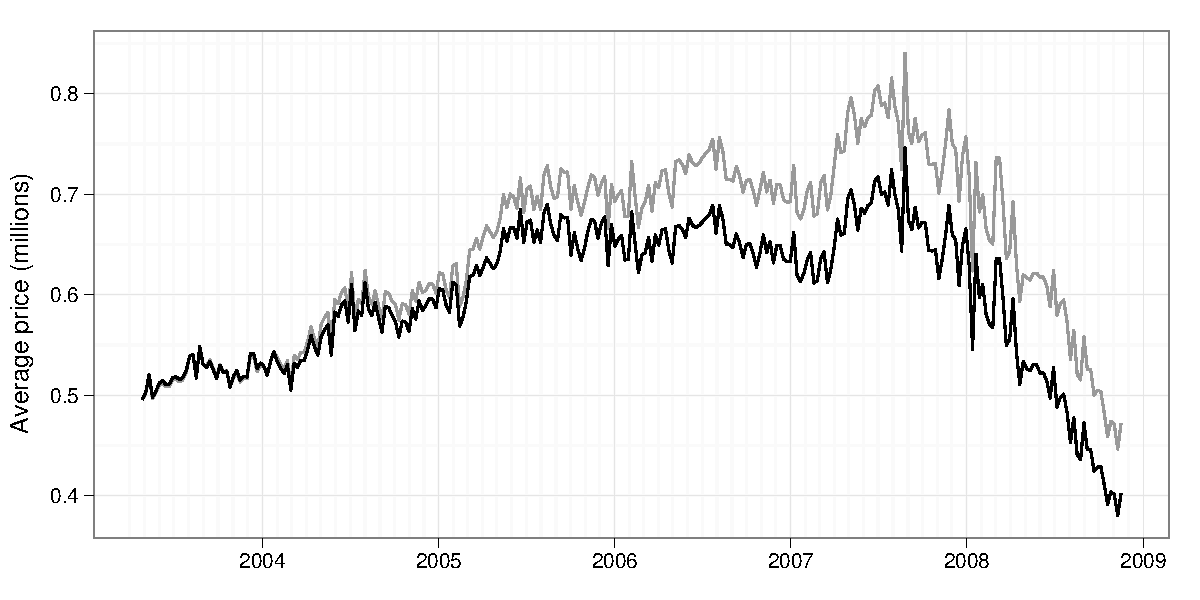
\includegraphics[width=0.5 \linewidth]{daily-price-adj}
  \caption{(Left) Inflation, indexed at 1 at start of series.  (Right) Inflation adjusted prices (black), and unadjusted prices (grey).  Failing to adjusting for inflation makes the rise look steeper, but has little effect on the decline.}
  \label{fig:inflation}
\end{figure}

\subsection{The rich get richer and the poor get poorer}

What is a decile?  How were they calculated?

Increasing disparity between top and bottom deciles.

\subsection{Accelerating foreclosures}

With the very cheap we see a large growth in the number of sales.

\subsection{Geographic differences}

City level break down.

Clustering.

\section{Watching city growth}

We can also use this data for an unexpected purpose.  Because the data is so dense and includes the year that the house was built, we can explore historical patterns of housing development.  This idea was inspired by truliaHindsight, \url{http://hindsight.trulia.com/}, but because we have the data in an unencumbered form we are much freer to experiment with the visualisation of this data.  They have much more data, 150,000 vs 27,000, but we can display more (they display at most 2000 points at once), and we can do more sophisticated analyses.

We'll overlay the data on a map of San Francisco from openstreetmap.

Histogram of year built.

You can see features like golden gate park and so on.

\section{Conclusions}

All the tools we use are open source: you can download them and replicate our work yourselves.  The principle of reproducible research (cite Gentleman and Temple Lang) paper is very important for science - we provide enough detail that you can follow out work every step of the way, and you can run a script to reproduce exactly what we did.  A little tricky because working on this data analysis also lead us to develop some new tools, and it takes some time for these to trickle into released versions.  If you have problems running the code we released, please let us know!  Data analysis like software development.  Local caches to speed things up and to provide some backup if the original sources go down.

Tension with interactive tools: they are great for discovery, but bad for reproducibility.  Once you have discovered something in your interactive tool, you need to be able to reproduce it independently so that others can see it too.  Area of active research (cite Heer's work).  Also need to note your findings as you go along - no way to do this purely in code.  If you read the code on the website you'll see we've used comments to note down what we see and the analysis follows a fairly logical flow.  This is different to what happens in practice - there are many blind alleys that didn't make the final cut.  We rely on the rcs system to keep these, although currently lacking tools to easily search past versions and see the wrong paths that we went down.

Tools: shell (wget, awk); R (ggplot2, plyr, reshape).

Note about graphics: can churn out rough versions for exploration very quickly - takes more time to polish them for publication.  Clarify story, remove extraneous elements and ensure that it supports the text.



\bibliography{references}

\end{document}
